\section{Simulated Dataset}\hfill

A sample of 100k $pp \rightarrow HH$ events were generated using MADGRAPH\_AMC@NLO~\cite{Alwall_2014} and showered through $H \rightarrow b\bar{b}$ channel using Pythia8~\cite{bierlich2022comprehensiveguidephysicsusage}. As each hard scatter process is showered in Pythia, pileup processes are overlaid using SoftQCD:inelastic generated with the A14 central tune with NNPDF2.3LO~\cite{bierlich2022comprehensiveguidephysicsusage}. The average number of pileup processes are controlled by parameter $\left<\mu\right>$ which follows a poisson distribution. Each pileup vertex undergoes gaussian smearing where the width in the x and y directions, representing the beam width, are 0.3mm and the spread in the z direction is 50mm. Stable final state particles are then passed to FastJet~\cite{Cacciari_2012} to be cluster into jets using $anti-k_t$ algorithm~\cite{Cacciari_2008} with R=0.4 and minimum $p_T$ of 25 GeV. \\

\begin{figure}[h]
\centering
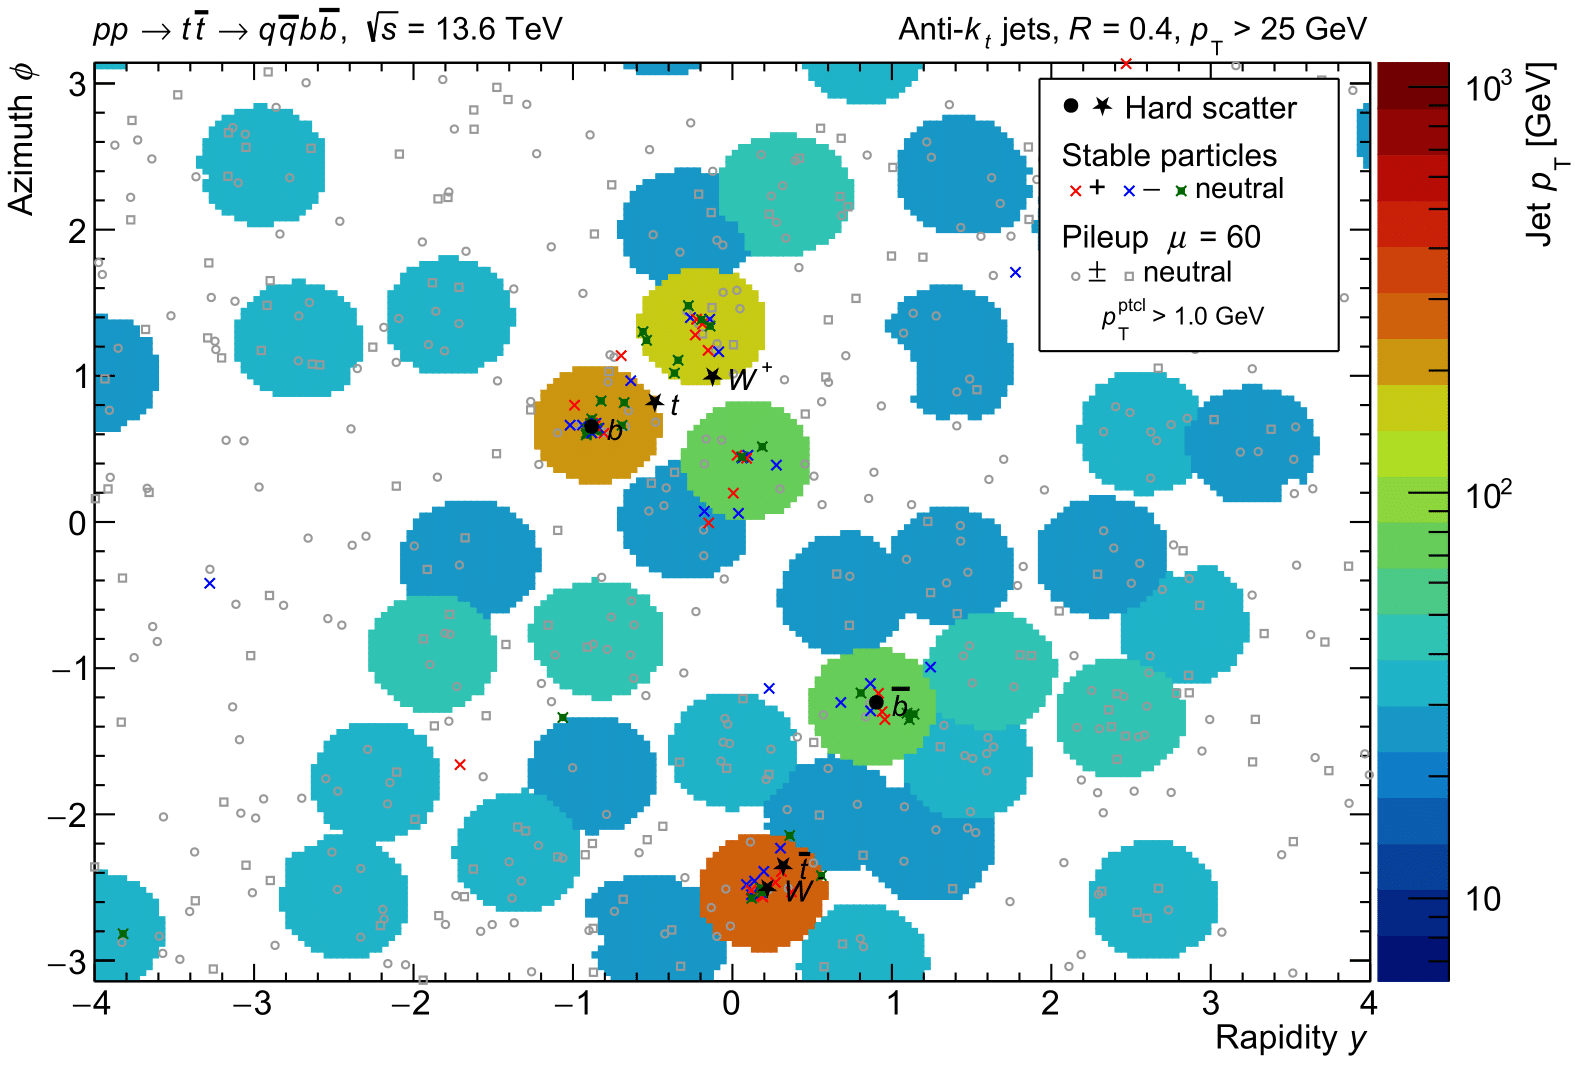
\includegraphics[width=0.65\textwidth]{Event}
\caption{An example of a simulated event of $pp \rightarrow t\bar{t}$ decaying hadronically at $\left< \mu \right> =60$.}
\end{figure}

To incorporate detector limitations, neutral particles and particles below 400 MeV were cut from the training dataset. After cuts, the dataset contains 500k jets and 10M particles. However, it is important to note that the jets studied in this paper are not calorimeter jets, but instead more idealistic track-jets. The results from this study offer the best-case scenario when tracks can be perfectly assigned the correct vertex, and the performance would be expected to degrade slightly in realistic detector conditions.